\documentclass[1p]{elsarticle_modified}
%\bibliographystyle{elsarticle-num}

%\usepackage[colorlinks]{hyperref}
%\usepackage{abbrmath_seonhwa} %\Abb, \Ascr, \Acal ,\Abf, \Afrak
\usepackage{amsfonts}
\usepackage{amssymb}
\usepackage{amsmath}
\usepackage{amsthm}
\usepackage{scalefnt}
\usepackage{amsbsy}
\usepackage{kotex}
\usepackage{caption}
\usepackage{subfig}
\usepackage{color}
\usepackage{graphicx}
\usepackage{xcolor} %% white, black, red, green, blue, cyan, magenta, yellow
\usepackage{float}
\usepackage{setspace}
\usepackage{hyperref}

\usepackage{tikz}
\usetikzlibrary{arrows}

\usepackage{multirow}
\usepackage{array} % fixed length table
\usepackage{hhline}

%%%%%%%%%%%%%%%%%%%%%
\makeatletter
\renewcommand*\env@matrix[1][\arraystretch]{%
	\edef\arraystretch{#1}%
	\hskip -\arraycolsep
	\let\@ifnextchar\new@ifnextchar
	\array{*\c@MaxMatrixCols c}}
\makeatother %https://tex.stackexchange.com/questions/14071/how-can-i-increase-the-line-spacing-in-a-matrix
%%%%%%%%%%%%%%%

\usepackage[normalem]{ulem}

\newcommand{\msout}[1]{\ifmmode\text{\sout{\ensuremath{#1}}}\else\sout{#1}\fi}
%SOURCE: \msout is \stkout macro in https://tex.stackexchange.com/questions/20609/strikeout-in-math-mode

\newcommand{\cancel}[1]{
	\ifmmode
	{\color{red}\msout{#1}}
	\else
	{\color{red}\sout{#1}}
	\fi
}

\newcommand{\add}[1]{
	{\color{blue}\uwave{#1}}
}

\newcommand{\replace}[2]{
	\ifmmode
	{\color{red}\msout{#1}}{\color{blue}\uwave{#2}}
	\else
	{\color{red}\sout{#1}}{\color{blue}\uwave{#2}}
	\fi
}

\newcommand{\Sol}{\mathcal{S}} %segment
\newcommand{\D}{D} %diagram
\newcommand{\A}{\mathcal{A}} %arc


%%%%%%%%%%%%%%%%%%%%%%%%%%%%%5 test

\def\sl{\operatorname{\textup{SL}}(2,\Cbb)}
\def\psl{\operatorname{\textup{PSL}}(2,\Cbb)}
\def\quan{\mkern 1mu \triangleright \mkern 1mu}

\theoremstyle{definition}
\newtheorem{thm}{Theorem}[section]
\newtheorem{prop}[thm]{Proposition}
\newtheorem{lem}[thm]{Lemma}
\newtheorem{ques}[thm]{Question}
\newtheorem{cor}[thm]{Corollary}
\newtheorem{defn}[thm]{Definition}
\newtheorem{exam}[thm]{Example}
\newtheorem{rmk}[thm]{Remark}
\newtheorem{alg}[thm]{Algorithm}

\newcommand{\I}{\sqrt{-1}}
\begin{document}

%\begin{frontmatter}
%
%\title{Boundary parabolic representations of knots up to 8 crossings}
%
%%% Group authors per affiliation:
%\author{Yunhi Cho} 
%\address{Department of Mathematics, University of Seoul, Seoul, Korea}
%\ead{yhcho@uos.ac.kr}
%
%
%\author{Seonhwa Kim} %\fnref{s_kim}}
%\address{Center for Geometry and Physics, Institute for Basic Science, Pohang, 37673, Korea}
%\ead{ryeona17@ibs.re.kr}
%
%\author{Hyuk Kim}
%\address{Department of Mathematical Sciences, Seoul National University, Seoul 08826, Korea}
%\ead{hyukkim@snu.ac.kr}
%
%\author{Seokbeom Yoon}
%\address{Department of Mathematical Sciences, Seoul National University, Seoul, 08826,  Korea}
%\ead{sbyoon15@snu.ac.kr}
%
%\begin{abstract}
%We find all boundary parabolic representation of knots up to 8 crossings.
%
%\end{abstract}
%\begin{keyword}
%    \MSC[2010] 57M25 
%\end{keyword}
%
%\end{frontmatter}

%\linenumbers
%\tableofcontents
%
\newcommand\colored[1]{\textcolor{white}{\rule[-0.35ex]{0.8em}{1.4ex}}\kern-0.8em\color{red} #1}%
%\newcommand\colored[1]{\textcolor{white}{ #1}\kern-2.17ex	\textcolor{white}{ #1}\kern-1.81ex	\textcolor{white}{ #1}\kern-2.15ex\color{red}#1	}

{\Large $\underline{12n_{0694}~(K12n_{0694})}$}

\setlength{\tabcolsep}{10pt}
\renewcommand{\arraystretch}{1.6}
\vspace{1cm}\begin{tabular}{m{100pt}>{\centering\arraybackslash}m{274pt}}
\multirow{5}{120pt}{
	\centering
	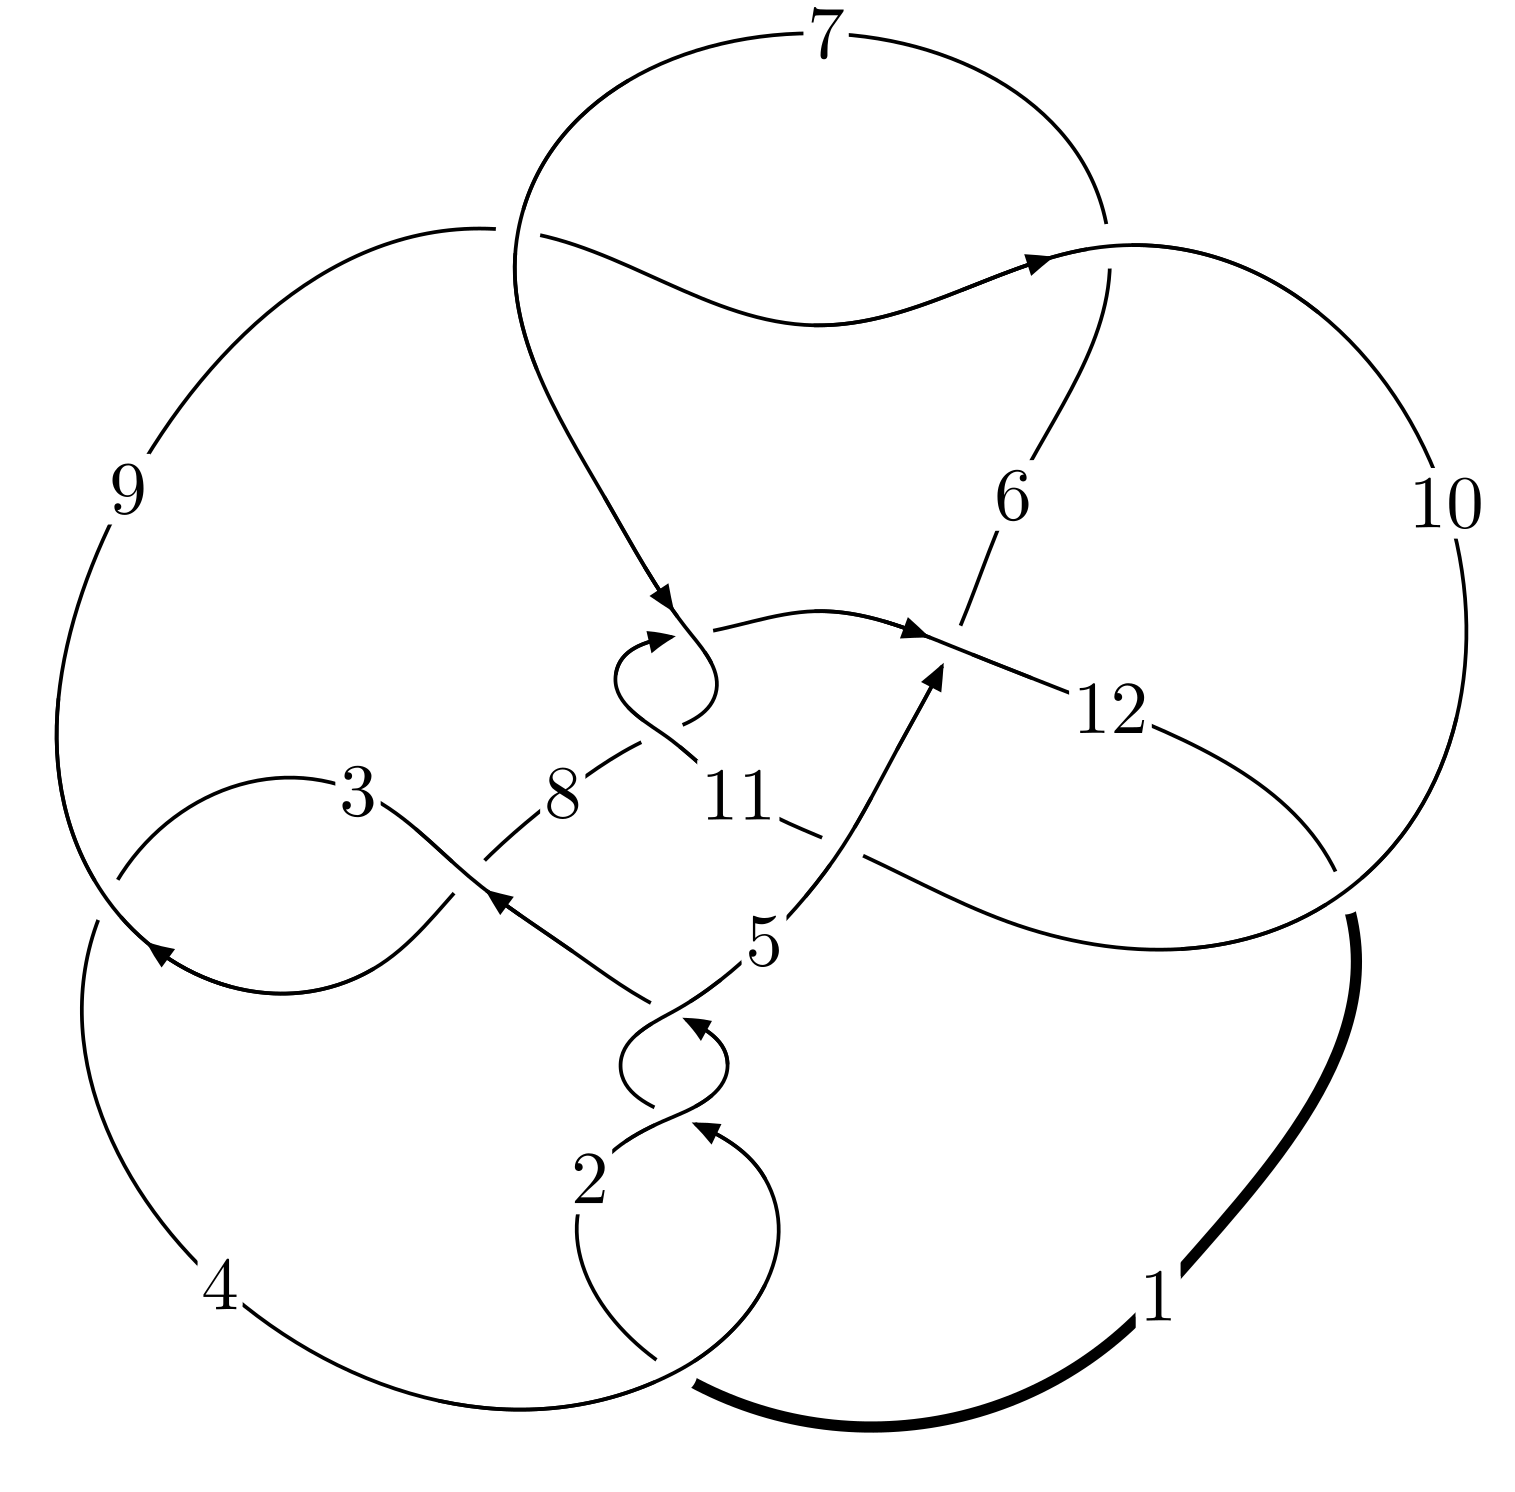
\includegraphics[width=112pt]{../../../GIT/diagram.site/Diagrams/png/2783_12n_0694.png}\\
\ \ \ A knot diagram\footnotemark}&
\allowdisplaybreaks
\textbf{Linearized knot diagam} \\
\cline{2-2}
 &
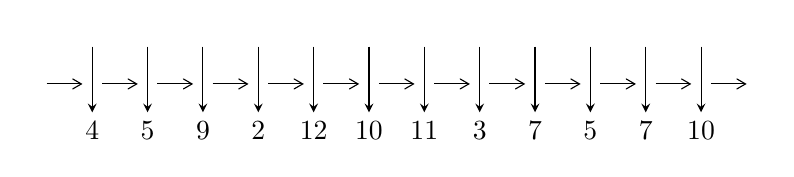
\begin{tikzpicture}[x=20pt, y=17pt]
	% nodes
	\node (C0) at (0, 0) {};
	\node (C1) at (1, 0) {};
	\node (C1U) at (1, +1) {};
	\node (C1D) at (1, -1) {4};

	\node (C2) at (2, 0) {};
	\node (C2U) at (2, +1) {};
	\node (C2D) at (2, -1) {5};

	\node (C3) at (3, 0) {};
	\node (C3U) at (3, +1) {};
	\node (C3D) at (3, -1) {9};

	\node (C4) at (4, 0) {};
	\node (C4U) at (4, +1) {};
	\node (C4D) at (4, -1) {2};

	\node (C5) at (5, 0) {};
	\node (C5U) at (5, +1) {};
	\node (C5D) at (5, -1) {12};

	\node (C6) at (6, 0) {};
	\node (C6U) at (6, +1) {};
	\node (C6D) at (6, -1) {10};

	\node (C7) at (7, 0) {};
	\node (C7U) at (7, +1) {};
	\node (C7D) at (7, -1) {11};

	\node (C8) at (8, 0) {};
	\node (C8U) at (8, +1) {};
	\node (C8D) at (8, -1) {3};

	\node (C9) at (9, 0) {};
	\node (C9U) at (9, +1) {};
	\node (C9D) at (9, -1) {7};

	\node (C10) at (10, 0) {};
	\node (C10U) at (10, +1) {};
	\node (C10D) at (10, -1) {5};

	\node (C11) at (11, 0) {};
	\node (C11U) at (11, +1) {};
	\node (C11D) at (11, -1) {7};

	\node (C12) at (12, 0) {};
	\node (C12U) at (12, +1) {};
	\node (C12D) at (12, -1) {10};
	\node (C13) at (13, 0) {};

	% arrows
	\draw[->,>={angle 60}]
	(C0) edge (C1) (C1) edge (C2) (C2) edge (C3) (C3) edge (C4) (C4) edge (C5) (C5) edge (C6) (C6) edge (C7) (C7) edge (C8) (C8) edge (C9) (C9) edge (C10) (C10) edge (C11) (C11) edge (C12) (C12) edge (C13) ;	\draw[->,>=stealth]
	(C1U) edge (C1D) (C2U) edge (C2D) (C3U) edge (C3D) (C4U) edge (C4D) (C5U) edge (C5D) (C6U) edge (C6D) (C7U) edge (C7D) (C8U) edge (C8D) (C9U) edge (C9D) (C10U) edge (C10D) (C11U) edge (C11D) (C12U) edge (C12D) ;
	\end{tikzpicture} \\
\hhline{~~} \\& 
\textbf{Solving Sequence} \\ \cline{2-2} 
 &
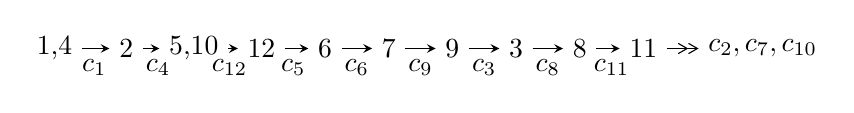
\begin{tikzpicture}[x=23pt, y=7pt]
	% node
	\node (A0) at (-1/8, 0) {1,4};
	\node (A1) at (1, 0) {2};
	\node (A2) at (33/16, 0) {5,10};
	\node (A3) at (25/8, 0) {12};
	\node (A4) at (33/8, 0) {6};
	\node (A5) at (41/8, 0) {7};
	\node (A6) at (49/8, 0) {9};
	\node (A7) at (57/8, 0) {3};
	\node (A8) at (65/8, 0) {8};
	\node (A9) at (73/8, 0) {11};
	\node (C1) at (1/2, -1) {$c_{1}$};
	\node (C2) at (3/2, -1) {$c_{4}$};
	\node (C3) at (21/8, -1) {$c_{12}$};
	\node (C4) at (29/8, -1) {$c_{5}$};
	\node (C5) at (37/8, -1) {$c_{6}$};
	\node (C6) at (45/8, -1) {$c_{9}$};
	\node (C7) at (53/8, -1) {$c_{3}$};
	\node (C8) at (61/8, -1) {$c_{8}$};
	\node (C9) at (69/8, -1) {$c_{11}$};
	\node (A10) at (11, 0) {$c_{2},c_{7},c_{10}$};

	% edge
	\draw[->,>=stealth]	
	(A0) edge (A1) (A1) edge (A2) (A2) edge (A3) (A3) edge (A4) (A4) edge (A5) (A5) edge (A6) (A6) edge (A7) (A7) edge (A8) (A8) edge (A9) ;
	\draw[->>,>={angle 60}]	
	(A9) edge (A10);
\end{tikzpicture} \\ 

\end{tabular} \\

\footnotetext{
The image of knot diagram is generated by the software ``\textbf{Draw programme}" developed by Andrew Bartholomew(\url{http://www.layer8.co.uk/maths/draw/index.htm\#Running-draw}), where we modified some parts for our purpose(\url{https://github.com/CATsTAILs/LinksPainter}).
}\phantom \\ \newline 
\centering \textbf{Ideals for irreducible components\footnotemark of $X_{\text{par}}$} 
 
\begin{align*}
I^u_{1}&=\langle 
5542348185 u^{14}+12483915678 u^{13}+\cdots+193710435976 b-48755007008,\\
\phantom{I^u_{1}}&\phantom{= \langle  }-57969081 u^{14}-531745184 u^{13}+\cdots+22789463056 a-38728287076,\\
\phantom{I^u_{1}}&\phantom{= \langle  }u^{15}+3 u^{14}+\cdots+60 u-16\rangle \\
I^u_{2}&=\langle 
u^4+2 u^3- u^2+b-2 u+2,\;u^4+3 u^3+a-6 u-4,\;u^5+4 u^4+3 u^3-4 u^2-4 u+1\rangle \\
I^u_{3}&=\langle 
13 a^3 u^2+2 a^3 u+3 a^2 u^2-9 a^3-3 a^2 u+24 u^2 a+a^2+11 a u+14 u^2+5 b-22 a-4 u+3,\\
\phantom{I^u_{3}}&\phantom{= \langle  }-2 a^3 u^2+a^4-2 a^3 u+2 a^2 u^2- a^3+3 a^2 u-32 u^2 a+4 a^2-53 a u+17 u^2-38 a+31 u+23,\;u^3+u^2-1\rangle \\
I^u_{4}&=\langle 
b- u,\;2 u^2+a+u-1,\;u^3- u+1\rangle \\
I^u_{5}&=\langle 
b-2 a+1,\;4 a^2-6 a+1,\;u-1\rangle \\
\\
\end{align*}
\raggedright * 5 irreducible components of $\dim_{\mathbb{C}}=0$, with total 37 representations.\\
\footnotetext{All coefficients of polynomials are rational numbers. But the coefficients are sometimes approximated in decimal forms when there is not enough margin.}
\newpage
\renewcommand{\arraystretch}{1}
\centering \section*{I. $I^u_{1}= \langle 5.54\times10^{9} u^{14}+1.25\times10^{10} u^{13}+\cdots+1.94\times10^{11} b-4.88\times10^{10},\;-5.80\times10^{7} u^{14}-5.32\times10^{8} u^{13}+\cdots+2.28\times10^{10} a-3.87\times10^{10},\;u^{15}+3 u^{14}+\cdots+60 u-16 \rangle$}
\flushleft \textbf{(i) Arc colorings}\\
\begin{tabular}{m{7pt} m{180pt} m{7pt} m{180pt} }
\flushright $a_{1}=$&$\begin{pmatrix}1\\0\end{pmatrix}$ \\
\flushright $a_{4}=$&$\begin{pmatrix}0\\u\end{pmatrix}$ \\
\flushright $a_{2}=$&$\begin{pmatrix}1\\u^2\end{pmatrix}$ \\
\flushright $a_{5}=$&$\begin{pmatrix}- u\\- u^3+u\end{pmatrix}$ \\
\flushright $a_{10}=$&$\begin{pmatrix}0.00254368 u^{14}+0.0233329 u^{13}+\cdots+0.0452708 u+1.69939\\-0.0286115 u^{14}-0.0644463 u^{13}+\cdots-1.99339 u+0.251690\end{pmatrix}$ \\
\flushright $a_{12}=$&$\begin{pmatrix}0.0380093 u^{14}+0.0802367 u^{13}+\cdots+2.56494 u+0.802099\\0.0511056 u^{14}+0.0966535 u^{13}+\cdots+3.44007 u-0.786612\end{pmatrix}$ \\
\flushright $a_{6}=$&$\begin{pmatrix}-0.0455457 u^{14}-0.0977825 u^{13}+\cdots-5.28838 u+0.536706\\-0.107164 u^{14}-0.218718 u^{13}+\cdots-7.08098 u+1.73158\end{pmatrix}$ \\
\flushright $a_{7}=$&$\begin{pmatrix}-0.00280296 u^{14}-0.0172477 u^{13}+\cdots-1.86151 u-0.654871\\-0.0399111 u^{14}-0.0794444 u^{13}+\cdots-2.27957 u+0.756192\end{pmatrix}$ \\
\flushright $a_{9}=$&$\begin{pmatrix}0.00251495 u^{14}+0.0394902 u^{13}+\cdots+0.759483 u+1.78965\\0.120131 u^{14}+0.203886 u^{13}+\cdots+7.47958 u-1.83534\end{pmatrix}$ \\
\flushright $a_{3}=$&$\begin{pmatrix}- u^2+1\\- u^4+2 u^2\end{pmatrix}$ \\
\flushright $a_{8}=$&$\begin{pmatrix}-0.00985312 u^{14}-0.00127324 u^{13}+\cdots+1.07235 u+1.36528\\0.102369 u^{14}+0.176801 u^{13}+\cdots+5.54963 u-1.50976\end{pmatrix}$ \\
\flushright $a_{11}=$&$\begin{pmatrix}0.0247410 u^{14}+0.0688107 u^{13}+\cdots+1.90500 u+1.26192\\-0.0282390 u^{14}-0.0646220 u^{13}+\cdots-2.23111 u+0.351338\end{pmatrix}$\\&\end{tabular}
\flushleft \textbf{(ii) Obstruction class $= -1$}\\~\\
\flushleft \textbf{(iii) Cusp Shapes $= \frac{22363926543}{45578926112} u^{14}+\frac{10216429583}{11394731528} u^{13}+\cdots+\frac{485831949075}{11394731528} u-\frac{73524844069}{2848682882}$}\\~\\
\newpage\renewcommand{\arraystretch}{1}
\flushleft \textbf{(iv) u-Polynomials at the component}\newline \\
\begin{tabular}{m{50pt}|m{274pt}}
Crossings & \hspace{64pt}u-Polynomials at each crossing \\
\hline $$\begin{aligned}c_{1},c_{2},c_{4}\end{aligned}$$&$\begin{aligned}
&u^{15}-3 u^{14}+\cdots+60 u+16
\end{aligned}$\\
\hline $$\begin{aligned}c_{3},c_{8}\end{aligned}$$&$\begin{aligned}
&u^{15}+8 u^{14}+\cdots-112 u-64
\end{aligned}$\\
\hline $$\begin{aligned}c_{5},c_{6},c_{9}\end{aligned}$$&$\begin{aligned}
&u^{15}+9 u^{12}+\cdots+7 u^2-1
\end{aligned}$\\
\hline $$\begin{aligned}c_{7},c_{10},c_{11}\end{aligned}$$&$\begin{aligned}
&u^{15}- u^{14}+\cdots+u+1
\end{aligned}$\\
\hline $$\begin{aligned}c_{12}\end{aligned}$$&$\begin{aligned}
&u^{15}-14 u^{14}+\cdots+68 u-8
\end{aligned}$\\
\hline
\end{tabular}\\~\\
\newpage\renewcommand{\arraystretch}{1}
\flushleft \textbf{(v) Riley Polynomials at the component}\newline \\
\begin{tabular}{m{50pt}|m{274pt}}
Crossings & \hspace{64pt}Riley Polynomials at each crossing \\
\hline $$\begin{aligned}c_{1},c_{2},c_{4}\end{aligned}$$&$\begin{aligned}
&y^{15}-15 y^{14}+\cdots+5232 y-256
\end{aligned}$\\
\hline $$\begin{aligned}c_{3},c_{8}\end{aligned}$$&$\begin{aligned}
&y^{15}-12 y^{14}+\cdots+41728 y-4096
\end{aligned}$\\
\hline $$\begin{aligned}c_{5},c_{6},c_{9}\end{aligned}$$&$\begin{aligned}
&y^{15}-4 y^{13}+\cdots+14 y-1
\end{aligned}$\\
\hline $$\begin{aligned}c_{7},c_{10},c_{11}\end{aligned}$$&$\begin{aligned}
&y^{15}+23 y^{14}+\cdots-23 y-1
\end{aligned}$\\
\hline $$\begin{aligned}c_{12}\end{aligned}$$&$\begin{aligned}
&y^{15}-68 y^{14}+\cdots+2576 y-64
\end{aligned}$\\
\hline
\end{tabular}\\~\\
\newpage\flushleft \textbf{(vi) Complex Volumes and Cusp Shapes}
$$\begin{array}{c|c|c}  
\text{Solutions to }I^u_{1}& \I (\text{vol} + \sqrt{-1}CS) & \text{Cusp shape}\\
 \hline 
\begin{aligned}
u &= -1.07635\phantom{ +0.000000I} \\
a &= \phantom{-}1.19704\phantom{ +0.000000I} \\
b &= \phantom{-}1.58782\phantom{ +0.000000I}\end{aligned}
 & -10.6859\phantom{ +0.000000I} & -41.6000\phantom{ +0.000000I} \\ \hline\begin{aligned}
u &= \phantom{-}1.178640 + 0.172680 I \\
a &= \phantom{-}0.627487 - 0.433643 I \\
b &= \phantom{-}0.282219 - 0.202348 I\end{aligned}
 & -1.55215 - 0.88269 I & -10.53205 + 2.04290 I \\ \hline\begin{aligned}
u &= \phantom{-}1.178640 - 0.172680 I \\
a &= \phantom{-}0.627487 + 0.433643 I \\
b &= \phantom{-}0.282219 + 0.202348 I\end{aligned}
 & -1.55215 + 0.88269 I & -10.53205 - 2.04290 I \\ \hline\begin{aligned}
u &= \phantom{-}0.160834 + 0.708843 I \\
a &= \phantom{-}0.014785 + 0.187812 I \\
b &= \phantom{-}0.520261 - 0.168254 I\end{aligned}
 & \phantom{-}1.32905 - 2.33965 I & -9.51656 + 6.09486 I \\ \hline\begin{aligned}
u &= \phantom{-}0.160834 - 0.708843 I \\
a &= \phantom{-}0.014785 - 0.187812 I \\
b &= \phantom{-}0.520261 + 0.168254 I\end{aligned}
 & \phantom{-}1.32905 + 2.33965 I & -9.51656 - 6.09486 I \\ \hline\begin{aligned}
u &= -1.360170 + 0.309898 I \\
a &= \phantom{-}0.509328 + 0.442124 I \\
b &= \phantom{-}0.714313 + 0.230460 I\end{aligned}
 & -3.48368 + 6.07143 I & -13.1701 - 10.7080 I \\ \hline\begin{aligned}
u &= -1.360170 - 0.309898 I \\
a &= \phantom{-}0.509328 - 0.442124 I \\
b &= \phantom{-}0.714313 - 0.230460 I\end{aligned}
 & -3.48368 - 6.07143 I & -13.1701 + 10.7080 I \\ \hline\begin{aligned}
u &= -0.12171 + 1.44460 I \\
a &= -0.280558 - 0.267780 I \\
b &= \phantom{-}2.37166 + 0.47398 I\end{aligned}
 & \phantom{-}9.74508 - 5.81410 I & -9.65717 + 3.18656 I \\ \hline\begin{aligned}
u &= -0.12171 - 1.44460 I \\
a &= -0.280558 + 0.267780 I \\
b &= \phantom{-}2.37166 - 0.47398 I\end{aligned}
 & \phantom{-}9.74508 + 5.81410 I & -9.65717 - 3.18656 I \\ \hline\begin{aligned}
u &= -1.42958 + 0.70949 I \\
a &= \phantom{-}1.01628 + 1.25193 I \\
b &= \phantom{-}2.03512 - 0.49412 I\end{aligned}
 & \phantom{-}5.6640 + 13.2045 I & -12.63072 - 5.98469 I\\
 \hline 
 \end{array}$$\newpage$$\begin{array}{c|c|c}  
\text{Solutions to }I^u_{1}& \I (\text{vol} + \sqrt{-1}CS) & \text{Cusp shape}\\
 \hline 
\begin{aligned}
u &= -1.42958 - 0.70949 I \\
a &= \phantom{-}1.01628 - 1.25193 I \\
b &= \phantom{-}2.03512 + 0.49412 I\end{aligned}
 & \phantom{-}5.6640 - 13.2045 I & -12.63072 + 5.98469 I \\ \hline\begin{aligned}
u &= \phantom{-}0.219796\phantom{ +0.000000I} \\
a &= \phantom{-}1.78361\phantom{ +0.000000I} \\
b &= -0.198958\phantom{ +0.000000I}\end{aligned}
 & -0.592779\phantom{ +0.000000I} & -16.9910\phantom{ +0.000000I} \\ \hline\begin{aligned}
u &= \phantom{-}1.68228 + 0.91262 I \\
a &= \phantom{-}0.793163 - 0.925065 I \\
b &= \phantom{-}3.00988 + 0.43262 I\end{aligned}
 & \phantom{-}4.36534 - 2.50283 I & -8.50423 + 2.90053 I \\ \hline\begin{aligned}
u &= \phantom{-}1.68228 - 0.91262 I \\
a &= \phantom{-}0.793163 + 0.925065 I \\
b &= \phantom{-}3.00988 - 0.43262 I\end{aligned}
 & \phantom{-}4.36534 + 2.50283 I & -8.50423 - 2.90053 I \\ \hline\begin{aligned}
u &= -2.36403\phantom{ +0.000000I} \\
a &= -1.34162\phantom{ +0.000000I} \\
b &= -5.25577\phantom{ +0.000000I}\end{aligned}
 & -19.2116\phantom{ +0.000000I} & \phantom{-}16.8620\phantom{ +0.000000I}\\
 \hline 
 \end{array}$$\newpage\newpage\renewcommand{\arraystretch}{1}
\centering \section*{II. $I^u_{2}= \langle u^4+2 u^3- u^2+b-2 u+2,\;u^4+3 u^3+a-6 u-4,\;u^5+4 u^4+3 u^3-4 u^2-4 u+1 \rangle$}
\flushleft \textbf{(i) Arc colorings}\\
\begin{tabular}{m{7pt} m{180pt} m{7pt} m{180pt} }
\flushright $a_{1}=$&$\begin{pmatrix}1\\0\end{pmatrix}$ \\
\flushright $a_{4}=$&$\begin{pmatrix}0\\u\end{pmatrix}$ \\
\flushright $a_{2}=$&$\begin{pmatrix}1\\u^2\end{pmatrix}$ \\
\flushright $a_{5}=$&$\begin{pmatrix}- u\\- u^3+u\end{pmatrix}$ \\
\flushright $a_{10}=$&$\begin{pmatrix}- u^4-3 u^3+6 u+4\\- u^4-2 u^3+u^2+2 u-2\end{pmatrix}$ \\
\flushright $a_{12}=$&$\begin{pmatrix}-2 u^4-5 u^3+u^2+10 u+7\\-4 u^4-7 u^3+4 u^2+7 u-4\end{pmatrix}$ \\
\flushright $a_{6}=$&$\begin{pmatrix}4 u^4+17 u^3+17 u^2-7 u-12\\-2 u^4-6 u^3-3 u^2+3 u+3\end{pmatrix}$ \\
\flushright $a_{7}=$&$\begin{pmatrix}2 u^4+8 u^3+7 u^2-4 u-5\\- u^4-3 u^3- u^2+2 u+1\end{pmatrix}$ \\
\flushright $a_{9}=$&$\begin{pmatrix}u^3+2 u^2- u-2\\-2 u^4-5 u^3+u^2+6 u-1\end{pmatrix}$ \\
\flushright $a_{3}=$&$\begin{pmatrix}- u^2+1\\- u^4+2 u^2\end{pmatrix}$ \\
\flushright $a_{8}=$&$\begin{pmatrix}3 u^4+7 u^3- u^2-8 u\\6 u^4+10 u^3-5 u^2-12 u+3\end{pmatrix}$ \\
\flushright $a_{11}=$&$\begin{pmatrix}- u^4-2 u^3+u^2+5 u+4\\-4 u^4-7 u^3+4 u^2+7 u-3\end{pmatrix}$\\&\end{tabular}
\flushleft \textbf{(ii) Obstruction class $= 1$}\\~\\
\flushleft \textbf{(iii) Cusp Shapes $= -10 u^4-33 u^3-29 u^2+3 u-6$}\\~\\
\newpage\renewcommand{\arraystretch}{1}
\flushleft \textbf{(iv) u-Polynomials at the component}\newline \\
\begin{tabular}{m{50pt}|m{274pt}}
Crossings & \hspace{64pt}u-Polynomials at each crossing \\
\hline $$\begin{aligned}c_{1},c_{2}\end{aligned}$$&$\begin{aligned}
&u^5+4 u^4+3 u^3-4 u^2-4 u+1
\end{aligned}$\\
\hline $$\begin{aligned}c_{3}\end{aligned}$$&$\begin{aligned}
&u^5-6 u^3+11 u^2-6 u+1
\end{aligned}$\\
\hline $$\begin{aligned}c_{4}\end{aligned}$$&$\begin{aligned}
&u^5-4 u^4+3 u^3+4 u^2-4 u-1
\end{aligned}$\\
\hline $$\begin{aligned}c_{5},c_{9}\end{aligned}$$&$\begin{aligned}
&u^5+u^4- u^3-2 u^2- u+1
\end{aligned}$\\
\hline $$\begin{aligned}c_{6}\end{aligned}$$&$\begin{aligned}
&u^5- u^4- u^3+2 u^2- u-1
\end{aligned}$\\
\hline $$\begin{aligned}c_{7},c_{10}\end{aligned}$$&$\begin{aligned}
&u^5+u^4-2 u^3+u^2+u-1
\end{aligned}$\\
\hline $$\begin{aligned}c_{8}\end{aligned}$$&$\begin{aligned}
&u^5-6 u^3-11 u^2-6 u-1
\end{aligned}$\\
\hline $$\begin{aligned}c_{11}\end{aligned}$$&$\begin{aligned}
&u^5- u^4-2 u^3- u^2+u+1
\end{aligned}$\\
\hline $$\begin{aligned}c_{12}\end{aligned}$$&$\begin{aligned}
&u^5+10 u^4+34 u^3+55 u^2+46 u+17
\end{aligned}$\\
\hline
\end{tabular}\\~\\
\newpage\renewcommand{\arraystretch}{1}
\flushleft \textbf{(v) Riley Polynomials at the component}\newline \\
\begin{tabular}{m{50pt}|m{274pt}}
Crossings & \hspace{64pt}Riley Polynomials at each crossing \\
\hline $$\begin{aligned}c_{1},c_{2},c_{4}\end{aligned}$$&$\begin{aligned}
&y^5-10 y^4+33 y^3-48 y^2+24 y-1
\end{aligned}$\\
\hline $$\begin{aligned}c_{3},c_{8}\end{aligned}$$&$\begin{aligned}
&y^5-12 y^4+24 y^3-49 y^2+14 y-1
\end{aligned}$\\
\hline $$\begin{aligned}c_{5},c_{6},c_{9}\end{aligned}$$&$\begin{aligned}
&y^5-3 y^4+3 y^3-4 y^2+5 y-1
\end{aligned}$\\
\hline $$\begin{aligned}c_{7},c_{10},c_{11}\end{aligned}$$&$\begin{aligned}
&y^5-5 y^4+4 y^3-3 y^2+3 y-1
\end{aligned}$\\
\hline $$\begin{aligned}c_{12}\end{aligned}$$&$\begin{aligned}
&y^5-32 y^4+148 y^3-237 y^2+246 y-289
\end{aligned}$\\
\hline
\end{tabular}\\~\\
\newpage\flushleft \textbf{(vi) Complex Volumes and Cusp Shapes}
$$\begin{array}{c|c|c}  
\text{Solutions to }I^u_{2}& \I (\text{vol} + \sqrt{-1}CS) & \text{Cusp shape}\\
 \hline 
\begin{aligned}
u &= \phantom{-}0.935978\phantom{ +0.000000I} \\
a &= \phantom{-}6.38849\phantom{ +0.000000I} \\
b &= -1.65940\phantom{ +0.000000I}\end{aligned}
 & -5.47443\phantom{ +0.000000I} & -63.3310\phantom{ +0.000000I} \\ \hline\begin{aligned}
u &= -1.41748 + 0.38647 I \\
a &= -0.124879 - 0.421155 I \\
b &= -0.807993 - 0.790836 I\end{aligned}
 & -3.56702 + 5.27138 I & -13.75047 - 1.28258 I \\ \hline\begin{aligned}
u &= -1.41748 - 0.38647 I \\
a &= -0.124879 + 0.421155 I \\
b &= -0.807993 + 0.790836 I\end{aligned}
 & -3.56702 - 5.27138 I & -13.75047 + 1.28258 I \\ \hline\begin{aligned}
u &= \phantom{-}0.213816\phantom{ +0.000000I} \\
a &= \phantom{-}5.25148\phantom{ +0.000000I} \\
b &= -1.54829\phantom{ +0.000000I}\end{aligned}
 & -4.24110\phantom{ +0.000000I} & -7.02780\phantom{ +0.000000I} \\ \hline\begin{aligned}
u &= -2.31483\phantom{ +0.000000I} \\
a &= -1.39021\phantom{ +0.000000I} \\
b &= -5.17632\phantom{ +0.000000I}\end{aligned}
 & -19.3390\phantom{ +0.000000I} & -46.1400\phantom{ +0.000000I}\\
 \hline 
 \end{array}$$\newpage\newpage\renewcommand{\arraystretch}{1}
\centering \section*{III. $I^u_{3}= \langle 13 a^3 u^2+3 a^2 u^2+\cdots-22 a+3,\;-2 a^3 u^2+2 a^2 u^2+\cdots-38 a+23,\;u^3+u^2-1 \rangle$}
\flushleft \textbf{(i) Arc colorings}\\
\begin{tabular}{m{7pt} m{180pt} m{7pt} m{180pt} }
\flushright $a_{1}=$&$\begin{pmatrix}1\\0\end{pmatrix}$ \\
\flushright $a_{4}=$&$\begin{pmatrix}0\\u\end{pmatrix}$ \\
\flushright $a_{2}=$&$\begin{pmatrix}1\\u^2\end{pmatrix}$ \\
\flushright $a_{5}=$&$\begin{pmatrix}- u\\u^2+u-1\end{pmatrix}$ \\
\flushright $a_{10}=$&$\begin{pmatrix}a\\-2.60000 a^{3} u^{2}-0.600000 a^{2} u^{2}+\cdots+4.40000 a-0.600000\end{pmatrix}$ \\
\flushright $a_{12}=$&$\begin{pmatrix}-\frac{2}{5} a^3 u^2+\frac{1}{5} a^2 u^2+\cdots-\frac{2}{5} a-\frac{4}{5}\\-2.60000 a^{3} u^{2}-0.600000 a^{2} u^{2}+\cdots+4.40000 a-1.60000\end{pmatrix}$ \\
\flushright $a_{6}=$&$\begin{pmatrix}- a^3 u^2-\frac{3}{5} a^2 u^2+\cdots- a-\frac{3}{5}\\\frac{7}{5} a^3 u^2+\frac{8}{5} a^2 u^2+\cdots-\frac{18}{5} a-\frac{17}{5}\end{pmatrix}$ \\
\flushright $a_{7}=$&$\begin{pmatrix}-\frac{4}{5} a^2 u^2-\frac{2}{5} u^2+\cdots+\frac{2}{5} a^2+\frac{6}{5}\\\frac{9}{5} a^3 u^2+\frac{2}{5} a^2 u^2+\cdots-\frac{11}{5} a+\frac{2}{5}\end{pmatrix}$ \\
\flushright $a_{9}=$&$\begin{pmatrix}- u\\2 u^2+u-2\end{pmatrix}$ \\
\flushright $a_{3}=$&$\begin{pmatrix}- u^2+1\\u^2- u+1\end{pmatrix}$ \\
\flushright $a_{8}=$&$\begin{pmatrix}-2 u+1\\5 u^2+2 u-4\end{pmatrix}$ \\
\flushright $a_{11}=$&$\begin{pmatrix}\frac{2}{5} a^3 u^2+\frac{7}{5} a^2 u^2+\cdots-\frac{13}{5} a-\frac{18}{5}\\-7.40000 a^{3} u^{2}-2.40000 a^{2} u^{2}+\cdots+15.6000 a+1.60000\end{pmatrix}$\\&\end{tabular}
\flushleft \textbf{(ii) Obstruction class $= -1$}\\~\\
\flushleft \textbf{(iii) Cusp Shapes $= -4 u-14$}\\~\\
\newpage\renewcommand{\arraystretch}{1}
\flushleft \textbf{(iv) u-Polynomials at the component}\newline \\
\begin{tabular}{m{50pt}|m{274pt}}
Crossings & \hspace{64pt}u-Polynomials at each crossing \\
\hline $$\begin{aligned}c_{1},c_{2},c_{4}\end{aligned}$$&$\begin{aligned}
&(u^3- u^2+1)^4
\end{aligned}$\\
\hline $$\begin{aligned}c_{3},c_{8}\end{aligned}$$&$\begin{aligned}
&(u^3- u^2+2 u-1)^4
\end{aligned}$\\
\hline $$\begin{aligned}c_{5},c_{6},c_{9}\end{aligned}$$&$\begin{aligned}
&u^{12}-3 u^{11}+\cdots-2 u-59
\end{aligned}$\\
\hline $$\begin{aligned}c_{7},c_{10},c_{11}\end{aligned}$$&$\begin{aligned}
&u^{12}+3 u^{11}+\cdots-314 u-121
\end{aligned}$\\
\hline $$\begin{aligned}c_{12}\end{aligned}$$&$\begin{aligned}
&(u^2+u-1)^6
\end{aligned}$\\
\hline
\end{tabular}\\~\\
\newpage\renewcommand{\arraystretch}{1}
\flushleft \textbf{(v) Riley Polynomials at the component}\newline \\
\begin{tabular}{m{50pt}|m{274pt}}
Crossings & \hspace{64pt}Riley Polynomials at each crossing \\
\hline $$\begin{aligned}c_{1},c_{2},c_{4}\end{aligned}$$&$\begin{aligned}
&(y^3- y^2+2 y-1)^4
\end{aligned}$\\
\hline $$\begin{aligned}c_{3},c_{8}\end{aligned}$$&$\begin{aligned}
&(y^3+3 y^2+2 y-1)^4
\end{aligned}$\\
\hline $$\begin{aligned}c_{5},c_{6},c_{9}\end{aligned}$$&$\begin{aligned}
&y^{12}- y^{11}+\cdots+5424 y+3481
\end{aligned}$\\
\hline $$\begin{aligned}c_{7},c_{10},c_{11}\end{aligned}$$&$\begin{aligned}
&y^{12}+11 y^{11}+\cdots-50196 y+14641
\end{aligned}$\\
\hline $$\begin{aligned}c_{12}\end{aligned}$$&$\begin{aligned}
&(y^2-3 y+1)^6
\end{aligned}$\\
\hline
\end{tabular}\\~\\
\newpage\flushleft \textbf{(vi) Complex Volumes and Cusp Shapes}
$$\begin{array}{c|c|c}  
\text{Solutions to }I^u_{3}& \I (\text{vol} + \sqrt{-1}CS) & \text{Cusp shape}\\
 \hline 
\begin{aligned}
u &= -0.877439 + 0.744862 I \\
a &= -0.037366 - 0.810507 I \\
b &= \phantom{-}0.618034\phantom{ +0.000000I}\end{aligned}
 & \phantom{-}6.97197 + 2.82812 I & -10.49024 - 2.97945 I \\ \hline\begin{aligned}
u &= -0.877439 + 0.744862 I \\
a &= -0.127901 - 1.361650 I \\
b &= -1.61803\phantom{ +0.000000I}\end{aligned}
 & -0.92371 + 2.82812 I & -10.49024 - 2.97945 I \\ \hline\begin{aligned}
u &= -0.877439 + 0.744862 I \\
a &= -0.397503 - 0.457922 I \\
b &= -1.61803\phantom{ +0.000000I}\end{aligned}
 & -0.92371 + 2.82812 I & -10.49024 - 2.97945 I \\ \hline\begin{aligned}
u &= -0.877439 + 0.744862 I \\
a &= \phantom{-}0.23805 + 1.50552 I \\
b &= \phantom{-}0.618034\phantom{ +0.000000I}\end{aligned}
 & \phantom{-}6.97197 + 2.82812 I & -10.49024 - 2.97945 I \\ \hline\begin{aligned}
u &= -0.877439 - 0.744862 I \\
a &= -0.037366 + 0.810507 I \\
b &= \phantom{-}0.618034\phantom{ +0.000000I}\end{aligned}
 & \phantom{-}6.97197 - 2.82812 I & -10.49024 + 2.97945 I \\ \hline\begin{aligned}
u &= -0.877439 - 0.744862 I \\
a &= -0.127901 + 1.361650 I \\
b &= -1.61803\phantom{ +0.000000I}\end{aligned}
 & -0.92371 - 2.82812 I & -10.49024 + 2.97945 I \\ \hline\begin{aligned}
u &= -0.877439 - 0.744862 I \\
a &= -0.397503 + 0.457922 I \\
b &= -1.61803\phantom{ +0.000000I}\end{aligned}
 & -0.92371 - 2.82812 I & -10.49024 + 2.97945 I \\ \hline\begin{aligned}
u &= -0.877439 - 0.744862 I \\
a &= \phantom{-}0.23805 - 1.50552 I \\
b &= \phantom{-}0.618034\phantom{ +0.000000I}\end{aligned}
 & \phantom{-}6.97197 - 2.82812 I & -10.49024 + 2.97945 I \\ \hline\begin{aligned}
u &= \phantom{-}0.754878\phantom{ +0.000000I} \\
a &= \phantom{-}0.603863\phantom{ +0.000000I} \\
b &= -1.61803\phantom{ +0.000000I}\end{aligned}
 & -5.06130\phantom{ +0.000000I} & -17.0200\phantom{ +0.000000I} \\ \hline\begin{aligned}
u &= \phantom{-}0.754878\phantom{ +0.000000I} \\
a &= -1.12774 + 4.03110 I \\
b &= \phantom{-}0.618034\phantom{ +0.000000I}\end{aligned}
 & \phantom{-}2.83439\phantom{ +0.000000I} & -17.0200\phantom{ +0.000000I}\\
 \hline 
 \end{array}$$\newpage$$\begin{array}{c|c|c}  
\text{Solutions to }I^u_{3}& \I (\text{vol} + \sqrt{-1}CS) & \text{Cusp shape}\\
 \hline 
\begin{aligned}
u &= \phantom{-}0.754878\phantom{ +0.000000I} \\
a &= -1.12774 - 4.03110 I \\
b &= \phantom{-}0.618034\phantom{ +0.000000I}\end{aligned}
 & \phantom{-}2.83439\phantom{ +0.000000I} & -17.0200\phantom{ +0.000000I} \\ \hline\begin{aligned}
u &= \phantom{-}0.754878\phantom{ +0.000000I} \\
a &= \phantom{-}5.30105\phantom{ +0.000000I} \\
b &= -1.61803\phantom{ +0.000000I}\end{aligned}
 & -5.06130\phantom{ +0.000000I} & -17.0200\phantom{ +0.000000I}\\
 \hline 
 \end{array}$$\newpage\newpage\renewcommand{\arraystretch}{1}
\centering \section*{IV. $I^u_{4}= \langle b- u,\;2 u^2+a+u-1,\;u^3- u+1 \rangle$}
\flushleft \textbf{(i) Arc colorings}\\
\begin{tabular}{m{7pt} m{180pt} m{7pt} m{180pt} }
\flushright $a_{1}=$&$\begin{pmatrix}1\\0\end{pmatrix}$ \\
\flushright $a_{4}=$&$\begin{pmatrix}0\\u\end{pmatrix}$ \\
\flushright $a_{2}=$&$\begin{pmatrix}1\\u^2\end{pmatrix}$ \\
\flushright $a_{5}=$&$\begin{pmatrix}- u\\1\end{pmatrix}$ \\
\flushright $a_{10}=$&$\begin{pmatrix}-2 u^2- u+1\\u\end{pmatrix}$ \\
\flushright $a_{12}=$&$\begin{pmatrix}u^2+u-1\\- u^2\end{pmatrix}$ \\
\flushright $a_{6}=$&$\begin{pmatrix}- u+1\\u^2- u+1\end{pmatrix}$ \\
\flushright $a_{7}=$&$\begin{pmatrix}- u^2+2\\u^2\end{pmatrix}$ \\
\flushright $a_{9}=$&$\begin{pmatrix}- u^2+1\\u^2\end{pmatrix}$ \\
\flushright $a_{3}=$&$\begin{pmatrix}- u^2+1\\u^2+u\end{pmatrix}$ \\
\flushright $a_{8}=$&$\begin{pmatrix}0\\- u\end{pmatrix}$ \\
\flushright $a_{11}=$&$\begin{pmatrix}- u^2- u\\- u^2+1\end{pmatrix}$\\&\end{tabular}
\flushleft \textbf{(ii) Obstruction class $= 1$}\\~\\
\flushleft \textbf{(iii) Cusp Shapes $= 2 u^2+5 u-14$}\\~\\
\newpage\renewcommand{\arraystretch}{1}
\flushleft \textbf{(iv) u-Polynomials at the component}\newline \\
\begin{tabular}{m{50pt}|m{274pt}}
Crossings & \hspace{64pt}u-Polynomials at each crossing \\
\hline $$\begin{aligned}c_{1},c_{2},c_{12}\end{aligned}$$&$\begin{aligned}
&u^3- u+1
\end{aligned}$\\
\hline $$\begin{aligned}c_{3}\end{aligned}$$&$\begin{aligned}
&(u+1)^3
\end{aligned}$\\
\hline $$\begin{aligned}c_{4}\end{aligned}$$&$\begin{aligned}
&u^3- u-1
\end{aligned}$\\
\hline $$\begin{aligned}c_{5},c_{9}\end{aligned}$$&$\begin{aligned}
&u^3+2 u^2+u+1
\end{aligned}$\\
\hline $$\begin{aligned}c_{6}\end{aligned}$$&$\begin{aligned}
&u^3-2 u^2+u-1
\end{aligned}$\\
\hline $$\begin{aligned}c_{7},c_{10}\end{aligned}$$&$\begin{aligned}
&u^3- u^2+2 u-1
\end{aligned}$\\
\hline $$\begin{aligned}c_{8}\end{aligned}$$&$\begin{aligned}
&(u-1)^3
\end{aligned}$\\
\hline $$\begin{aligned}c_{11}\end{aligned}$$&$\begin{aligned}
&u^3+u^2+2 u+1
\end{aligned}$\\
\hline
\end{tabular}\\~\\
\newpage\renewcommand{\arraystretch}{1}
\flushleft \textbf{(v) Riley Polynomials at the component}\newline \\
\begin{tabular}{m{50pt}|m{274pt}}
Crossings & \hspace{64pt}Riley Polynomials at each crossing \\
\hline $$\begin{aligned}c_{1},c_{2},c_{4}\\c_{12}\end{aligned}$$&$\begin{aligned}
&y^3-2 y^2+y-1
\end{aligned}$\\
\hline $$\begin{aligned}c_{3},c_{8}\end{aligned}$$&$\begin{aligned}
&(y-1)^3
\end{aligned}$\\
\hline $$\begin{aligned}c_{5},c_{6},c_{9}\end{aligned}$$&$\begin{aligned}
&y^3-2 y^2-3 y-1
\end{aligned}$\\
\hline $$\begin{aligned}c_{7},c_{10},c_{11}\end{aligned}$$&$\begin{aligned}
&y^3+3 y^2+2 y-1
\end{aligned}$\\
\hline
\end{tabular}\\~\\
\newpage\flushleft \textbf{(vi) Complex Volumes and Cusp Shapes}
$$\begin{array}{c|c|c}  
\text{Solutions to }I^u_{4}& \I (\text{vol} + \sqrt{-1}CS) & \text{Cusp shape}\\
 \hline 
\begin{aligned}
u &= \phantom{-}0.662359 + 0.562280 I \\
a &= \phantom{-}0.09252 - 2.05200 I \\
b &= \phantom{-}0.662359 + 0.562280 I\end{aligned}
 & \phantom{-}2.83014 - 0.94271 I & -10.44308 + 4.30112 I \\ \hline\begin{aligned}
u &= \phantom{-}0.662359 - 0.562280 I \\
a &= \phantom{-}0.09252 + 2.05200 I \\
b &= \phantom{-}0.662359 - 0.562280 I\end{aligned}
 & \phantom{-}2.83014 + 0.94271 I & -10.44308 - 4.30112 I \\ \hline\begin{aligned}
u &= -1.32472\phantom{ +0.000000I} \\
a &= -1.18504\phantom{ +0.000000I} \\
b &= -1.32472\phantom{ +0.000000I}\end{aligned}
 & -8.95014\phantom{ +0.000000I} & -17.1140\phantom{ +0.000000I}\\
 \hline 
 \end{array}$$\newpage\newpage\renewcommand{\arraystretch}{1}
\centering \section*{V. $I^u_{5}= \langle b-2 a+1,\;4 a^2-6 a+1,\;u-1 \rangle$}
\flushleft \textbf{(i) Arc colorings}\\
\begin{tabular}{m{7pt} m{180pt} m{7pt} m{180pt} }
\flushright $a_{1}=$&$\begin{pmatrix}1\\0\end{pmatrix}$ \\
\flushright $a_{4}=$&$\begin{pmatrix}0\\1\end{pmatrix}$ \\
\flushright $a_{2}=$&$\begin{pmatrix}1\\1\end{pmatrix}$ \\
\flushright $a_{5}=$&$\begin{pmatrix}-1\\0\end{pmatrix}$ \\
\flushright $a_{10}=$&$\begin{pmatrix}a\\2 a-1\end{pmatrix}$ \\
\flushright $a_{12}=$&$\begin{pmatrix}-2 a+\frac{3}{2}\\-2 a\end{pmatrix}$ \\
\flushright $a_{6}=$&$\begin{pmatrix}-3 a\\-6 a+1\end{pmatrix}$ \\
\flushright $a_{7}=$&$\begin{pmatrix}-0.5\\-2 a\end{pmatrix}$ \\
\flushright $a_{9}=$&$\begin{pmatrix}0\\-4 a\end{pmatrix}$ \\
\flushright $a_{3}=$&$\begin{pmatrix}0\\1\end{pmatrix}$ \\
\flushright $a_{8}=$&$\begin{pmatrix}0\\-4 a\end{pmatrix}$ \\
\flushright $a_{11}=$&$\begin{pmatrix}- a+1\\2 a-1\end{pmatrix}$\\&\end{tabular}
\flushleft \textbf{(ii) Obstruction class $= 1$}\\~\\
\flushleft \textbf{(iii) Cusp Shapes $= \frac{45}{2} a-20$}\\~\\
\newpage\renewcommand{\arraystretch}{1}
\flushleft \textbf{(iv) u-Polynomials at the component}\newline \\
\begin{tabular}{m{50pt}|m{274pt}}
Crossings & \hspace{64pt}u-Polynomials at each crossing \\
\hline $$\begin{aligned}c_{1},c_{2}\end{aligned}$$&$\begin{aligned}
&(u-1)^2
\end{aligned}$\\
\hline $$\begin{aligned}c_{3},c_{8}\end{aligned}$$&$\begin{aligned}
&u^2
\end{aligned}$\\
\hline $$\begin{aligned}c_{4}\end{aligned}$$&$\begin{aligned}
&(u+1)^2
\end{aligned}$\\
\hline $$\begin{aligned}c_{5},c_{6}\end{aligned}$$&$\begin{aligned}
&u^2-3 u+1
\end{aligned}$\\
\hline $$\begin{aligned}c_{7}\end{aligned}$$&$\begin{aligned}
&u^2+u-1
\end{aligned}$\\
\hline $$\begin{aligned}c_{9}\end{aligned}$$&$\begin{aligned}
&u^2+3 u+1
\end{aligned}$\\
\hline $$\begin{aligned}c_{10},c_{11},c_{12}\end{aligned}$$&$\begin{aligned}
&u^2- u-1
\end{aligned}$\\
\hline
\end{tabular}\\~\\
\newpage\renewcommand{\arraystretch}{1}
\flushleft \textbf{(v) Riley Polynomials at the component}\newline \\
\begin{tabular}{m{50pt}|m{274pt}}
Crossings & \hspace{64pt}Riley Polynomials at each crossing \\
\hline $$\begin{aligned}c_{1},c_{2},c_{4}\end{aligned}$$&$\begin{aligned}
&(y-1)^2
\end{aligned}$\\
\hline $$\begin{aligned}c_{3},c_{8}\end{aligned}$$&$\begin{aligned}
&y^2
\end{aligned}$\\
\hline $$\begin{aligned}c_{5},c_{6},c_{9}\end{aligned}$$&$\begin{aligned}
&y^2-7 y+1
\end{aligned}$\\
\hline $$\begin{aligned}c_{7},c_{10},c_{11}\\c_{12}\end{aligned}$$&$\begin{aligned}
&y^2-3 y+1
\end{aligned}$\\
\hline
\end{tabular}\\~\\
\newpage\flushleft \textbf{(vi) Complex Volumes and Cusp Shapes}
$$\begin{array}{c|c|c}  
\text{Solutions to }I^u_{5}& \I (\text{vol} + \sqrt{-1}CS) & \text{Cusp shape}\\
 \hline 
\begin{aligned}
u &= \phantom{-}1.00000\phantom{ +0.000000I} \\
a &= \phantom{-}1.30902\phantom{ +0.000000I} \\
b &= \phantom{-}1.61803\phantom{ +0.000000I}\end{aligned}
 & -10.5276\phantom{ +0.000000I} & \phantom{-}9.45290\phantom{ +0.000000I} \\ \hline\begin{aligned}
u &= \phantom{-}1.00000\phantom{ +0.000000I} \\
a &= \phantom{-}0.190983\phantom{ +0.000000I} \\
b &= -0.618034\phantom{ +0.000000I}\end{aligned}
 & -2.63189\phantom{ +0.000000I} & -15.7030\phantom{ +0.000000I}\\
 \hline 
 \end{array}$$\newpage
\newpage\renewcommand{\arraystretch}{1}
\centering \section*{ VI. u-Polynomials}
\begin{tabular}{m{50pt}|m{274pt}}
Crossings & \hspace{64pt}u-Polynomials at each crossing \\
\hline $$\begin{aligned}c_{1},c_{2}\end{aligned}$$&$\begin{aligned}
&(u-1)^2(u^3- u+1)(u^3- u^2+1)^4(u^5+4 u^4+3 u^3-4 u^2-4 u+1)\\
&\cdot(u^{15}-3 u^{14}+\cdots+60 u+16)
\end{aligned}$\\
\hline $$\begin{aligned}c_{3}\end{aligned}$$&$\begin{aligned}
&u^2(u+1)^3(u^3- u^2+2 u-1)^4(u^5-6 u^3+11 u^2-6 u+1)\\
&\cdot(u^{15}+8 u^{14}+\cdots-112 u-64)
\end{aligned}$\\
\hline $$\begin{aligned}c_{4}\end{aligned}$$&$\begin{aligned}
&(u+1)^2(u^3- u-1)(u^3- u^2+1)^4(u^5-4 u^4+3 u^3+4 u^2-4 u-1)\\
&\cdot(u^{15}-3 u^{14}+\cdots+60 u+16)
\end{aligned}$\\
\hline $$\begin{aligned}c_{5}\end{aligned}$$&$\begin{aligned}
&(u^2-3 u+1)(u^3+2 u^2+u+1)(u^5+u^4- u^3-2 u^2- u+1)\\
&\cdot(u^{12}-3 u^{11}+\cdots-2 u-59)(u^{15}+9 u^{12}+\cdots+7 u^2-1)
\end{aligned}$\\
\hline $$\begin{aligned}c_{6}\end{aligned}$$&$\begin{aligned}
&(u^2-3 u+1)(u^3-2 u^2+u-1)(u^5- u^4- u^3+2 u^2- u-1)\\
&\cdot(u^{12}-3 u^{11}+\cdots-2 u-59)(u^{15}+9 u^{12}+\cdots+7 u^2-1)
\end{aligned}$\\
\hline $$\begin{aligned}c_{7}\end{aligned}$$&$\begin{aligned}
&(u^2+u-1)(u^3- u^2+2 u-1)(u^5+u^4-2 u^3+u^2+u-1)\\
&\cdot(u^{12}+3 u^{11}+\cdots-314 u-121)(u^{15}- u^{14}+\cdots+u+1)
\end{aligned}$\\
\hline $$\begin{aligned}c_{8}\end{aligned}$$&$\begin{aligned}
&u^2(u-1)^3(u^3- u^2+2 u-1)^4(u^5-6 u^3-11 u^2-6 u-1)\\
&\cdot(u^{15}+8 u^{14}+\cdots-112 u-64)
\end{aligned}$\\
\hline $$\begin{aligned}c_{9}\end{aligned}$$&$\begin{aligned}
&(u^2+3 u+1)(u^3+2 u^2+u+1)(u^5+u^4- u^3-2 u^2- u+1)\\
&\cdot(u^{12}-3 u^{11}+\cdots-2 u-59)(u^{15}+9 u^{12}+\cdots+7 u^2-1)
\end{aligned}$\\
\hline $$\begin{aligned}c_{10}\end{aligned}$$&$\begin{aligned}
&(u^2- u-1)(u^3- u^2+2 u-1)(u^5+u^4-2 u^3+u^2+u-1)\\
&\cdot(u^{12}+3 u^{11}+\cdots-314 u-121)(u^{15}- u^{14}+\cdots+u+1)
\end{aligned}$\\
\hline $$\begin{aligned}c_{11}\end{aligned}$$&$\begin{aligned}
&(u^2- u-1)(u^3+u^2+2 u+1)(u^5- u^4-2 u^3- u^2+u+1)\\
&\cdot(u^{12}+3 u^{11}+\cdots-314 u-121)(u^{15}- u^{14}+\cdots+u+1)
\end{aligned}$\\
\hline $$\begin{aligned}c_{12}\end{aligned}$$&$\begin{aligned}
&(u^2- u-1)(u^2+u-1)^6(u^3- u+1)\\
&\cdot(u^5+10 u^4+\cdots+46 u+17)(u^{15}-14 u^{14}+\cdots+68 u-8)
\end{aligned}$\\
\hline
\end{tabular}\newpage\renewcommand{\arraystretch}{1}
\centering \section*{ VII. Riley Polynomials}
\begin{tabular}{m{50pt}|m{274pt}}
Crossings & \hspace{64pt}Riley Polynomials at each crossing \\
\hline $$\begin{aligned}c_{1},c_{2},c_{4}\end{aligned}$$&$\begin{aligned}
&(y-1)^2(y^3-2 y^2+y-1)(y^3- y^2+2 y-1)^4\\
&\cdot(y^5-10 y^4+\cdots+24 y-1)(y^{15}-15 y^{14}+\cdots+5232 y-256)
\end{aligned}$\\
\hline $$\begin{aligned}c_{3},c_{8}\end{aligned}$$&$\begin{aligned}
&y^2(y-1)^3(y^{3}+3 y^{2}+2 y-1)^{4}(y^{5}-12 y^{4}+\cdots+14 y-1)\\
&\cdot(y^{15}-12 y^{14}+\cdots+41728 y-4096)
\end{aligned}$\\
\hline $$\begin{aligned}c_{5},c_{6},c_{9}\end{aligned}$$&$\begin{aligned}
&(y^2-7 y+1)(y^3-2 y^2-3 y-1)(y^5-3 y^4+3 y^3-4 y^2+5 y-1)\\
&\cdot(y^{12}- y^{11}+\cdots+5424 y+3481)(y^{15}-4 y^{13}+\cdots+14 y-1)
\end{aligned}$\\
\hline $$\begin{aligned}c_{7},c_{10},c_{11}\end{aligned}$$&$\begin{aligned}
&(y^2-3 y+1)(y^3+3 y^2+2 y-1)(y^5-5 y^4+4 y^3-3 y^2+3 y-1)\\
&\cdot(y^{12}+11 y^{11}+\cdots-50196 y+14641)(y^{15}+23 y^{14}+\cdots-23 y-1)
\end{aligned}$\\
\hline $$\begin{aligned}c_{12}\end{aligned}$$&$\begin{aligned}
&(y^2-3 y+1)^7(y^3-2 y^2+y-1)\\
&\cdot(y^5-32 y^4+148 y^3-237 y^2+246 y-289)\\
&\cdot(y^{15}-68 y^{14}+\cdots+2576 y-64)
\end{aligned}$\\
\hline
\end{tabular}
\vskip 2pc
\end{document}